\documentclass{beamer}
\usecolortheme{wolverine}

% math stuff
\usepackage{amsmath}
\usepackage{amsthm}
\usepackage{amssymb}
\usepackage{xcolor}

\usepackage{float}
\usepackage{subcaption}

% to insert images
\usepackage{graphicx}

% to correctly insert stressed characters
\usepackage[T1]{fontenc}
\usepackage[utf8]{inputenc}

\usepackage{multirow}

% Bibliography
% \usepackage[style=alphabetic]{biblatex}
% \usepackage[nottoc]{tocbibind}
% \usepackage{bibentry}
% \setcounter{biburllcpenalty}{9000}
% \usepackage{nameref}
% \addbibresource{slides.bib}

% to put links in table of contents
\usepackage{hyperref}
\hypersetup{colorlinks=false, %set true if you want colored links
	linktoc=all,     %set to all if you
}

\usepackage{mathtools}

% Add symbols
% \usepackage{textcomp}

% Add command for Real and Z sets
% \usepackage{dsfont}
% \newcommand{\Rset}{$\mathds{R}$}
% \newcommand{\Zset}{$\mathds{Z}$}

% Code highlighting
% \usepackage{minted}
% \usemintedstyle{perldoc}
% \setminted{
%     frame=single,
%     breaklines,
% }

% tikz figures
\usepackage{tikzit}
\input{style.tikzstyles}

% number rounding
\usepackage{siunitx}
\sisetup{round-mode=places,round-precision=5}

\definecolor{myyellow}{RGB}{225, 225, 0}

\title{Thesis notes}
\date{6th April}

% any code between @(...)@ is escaped back to LaTeX
% \lstset{escapeinside={@(}{)@}}

% algorithms
\usepackage[ruled,vlined]{algorithm2e}

\newtheorem{theorem}{Theorem}

\begin{document}
\frame{\titlepage}

\begin{frame}[c]
	\frametitle{The echo chamber problem - notation}
	\begin{itemize}
		\item $G = (V, E ^{+}, E ^{-}) $ interaction graph
		\item $ \mathcal{C} $ set of contents
		\item $C \in \mathcal{C} $ content, $\mathcal{T} _{C} $ set of threads
		      associated with $C$. A thread $T \in \mathcal{T} _{C} $ is a
		      subgraph of $G$
		      % So $G = \bigcup _{C
		      % \in \mathcal{C} } \bigcup _{T \in \mathcal{T} _C} T $ union of all
		      % threads of all contents
		\item $U \subseteq V$ subset of users, $T[U]$ subgraph of $T$ induced
		      by $U$. $|T(U)|$ is the number of edges of this subgraph
	\end{itemize}
\end{frame}

\begin{frame}[c]
	\frametitle{The echo chamber problem - notation}
	\begin{itemize}
		\item $\eta(C)$ fraction of negative edges associated with $C$
		      (analogous definition for a thread $T$). Content (or thread)
		      controversial if $\eta \in [\alpha, 1]$
		\item $\hat{\mathcal{C} } \subseteq \mathcal{C} $ set of \textit{controversial}
		      contents

		\item $\mathcal{S} _C (U)$ set of \textit{non controversial} threads
		      induced by $U$, for \textit{controversial} contents, i.e.

			      {\small
				      \begin{equation}
					      \mathcal{S} _{C} (U) = \{ T[U] \; s.t. \; T[U] \; non \;
					      controversial, T \in \mathcal{T} _{C}, C
					      \in \hat{\mathcal{C}}, U \subseteq V\}
				      \end{equation}
			      }
	\end{itemize}

\end{frame}

\begin{frame}[c]
	\frametitle{The echo chamber problem}
	\textbf{Goal}: given an interaction graph $G$, find $U \subseteq V$ maximing

	\begin{equation}
		\xi (U) = \sum^{}_{C \in \hat{\mathcal{C}} } \sum^{}_{T[U] \in S_C (U)}
		| T[U] |
	\end{equation}

	The set of users maximing the expression is denoted as $\hat{U}$ and the
	corresponding score is $\xi(G)$
\end{frame}

\begin{frame}[c]
	\frametitle{An initial implementation}

	\begin{algorithm}[H]
		\SetAlgoLined
		% \KwResult{Write here the result }
		$U = \{$ random node $\}$\;
		\While{$\xi(U)$ can be increased by adding a node}{
			With probability $\beta $  {
					add to $U$ the node increasing more the score
					$\xi(U)$ (taking into account variations in $S_C (U)$)\;
				}
			With probability $(1 - \beta )$ remove from $U$ the node increasing less the
			score $\xi(U)$. This node will be ignored in the next iteration\;
		}
		\caption{Greedy approach}
	\end{algorithm}

\end{frame}

\begin{frame}[c]
	\frametitle{Another possible greedy approach}

	\begin{algorithm}[H]
		\SetAlgoLined
		% \KwResult{Write here the result }
		$U = \{$ all nodes $\}$\;
		$S$ = $\xi(U)$ \;
		\While{$U$ is not empty}{
			remove from $U$ the node contributing less to the score $\xi(U)$\;
			update $S$ if the current score is higher\;
		}
		\caption{Greedy approach}
	\end{algorithm}

\end{frame}


\begin{frame}[c]
	\frametitle{Computing exactly the score}

	\begin{equation}
		maximize\; \sum_{ij \in E(T_{k}), T_{k} \in \mathcal{T}_{C}, C \in
			\mathcal{\hat{C}} } x_{ij} ^{k}
	\end{equation}
	\begin{equation}
		x _{ij}^{k}  \leq y_i \quad\quad \forall ij \in E(T_{k}), T_{k} \in
		\mathcal{T}_{C}, C \in \mathcal{\hat{C}}
	\end{equation}
	\begin{equation}
		x _{ij} ^{k} \leq y_j \quad\quad \forall ij \in E(T_{k}), T_{k} \in
		\mathcal{T}_{C}, C \in \mathcal{\hat{C}}
	\end{equation}
	\begin{equation}
		x _{ij}^{k}  \leq z_k \quad\quad \forall ij \in E(T_k), T_k \in \mathcal{T} _{C}, C \in \hat{\mathcal{C} }
	\end{equation}
	\begin{equation}
		x _{ij} ^{k} \geq - 2 + y_i + y_j + z_k \quad\quad \forall ij \in E(T_k), T_k \in \mathcal{T} _{C}, C \in \hat{\mathcal{C} }
	\end{equation}
	\begin{equation}
		\sum^{}_{ij \in E^{-} (T_k)} x_{ij}^{k}  - \alpha \sum^{}_{ij \in E(T_k)}
		x_{ij} ^{k}  \leq 0 \quad\quad \forall T_{k} \in \mathcal{T} _{C}, C \in
		\hat{\mathcal{C}}
	\end{equation}
	% \begin{equation}
	%     \sum^{}_{ij \in E(T_{k} )} x_{ij} \leq N_{k} z_{k}
	% \end{equation}
	\begin{equation}
		y _{i} \in  \{0, 1\} \quad\quad \forall i \in V
	\end{equation}
	\begin{equation}
		0 \leq x _{ij} ^{k}  \leq 1 \quad\quad \forall ij \in E(T_{k}), T_{k} \in
		\mathcal{T}_{C}, C \in \mathcal{\hat{C}}
	\end{equation}
	\begin{equation}
		0 \leq z _{k} \leq 1 \quad\quad \forall T_{k} \in \mathcal{T} _{C}, C \in
		\hat{\mathcal{C}}
	\end{equation}
\end{frame}

\begin{frame}[c]
	\frametitle{Reconstructing solutions from relaxation results}

	\begin{algorithm}[H]
		\SetAlgoLined
		$E_{ordered} \coloneqq$ Edges ordered in descending order according to
		their value $x_{ij} $ \;
		$U \coloneqq \emptyset$ \;
		\ForEach{ $e_{ij}  \in E_{ordered} $}{
			Add $v_i$ and $v_{j} $ if not present in $U$\;
			Calculate $\xi(U)$ \;
		}
		\caption{Relaxation results reconstruction}
	\end{algorithm}

\end{frame}

\begin{frame}[c]
	\frametitle{Computing exactly the score - relaxation algorithm example}
	\begin{figure}
		\begin{center}
			\begin{subfigure}[b]{0.3\textwidth}
				\centering
				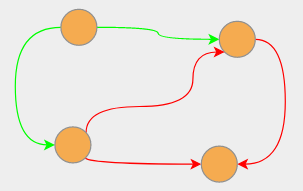
\includegraphics[width=\textwidth]{img/graph-example2-1.png}
				\caption{Original graph}
				\label{fig:img/graph-example2-1.png}
			\end{subfigure}
			\begin{subfigure}[b]{0.3\textwidth}
				\centering
				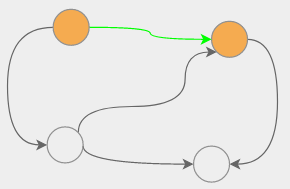
\includegraphics[width=\textwidth]{img/graph-example2-2.png}
				\caption{Integer solution}
				\label{fig:img/graph-example2-2.png}
			\end{subfigure}
			\begin{subfigure}[b]{0.3\textwidth}
				\centering
				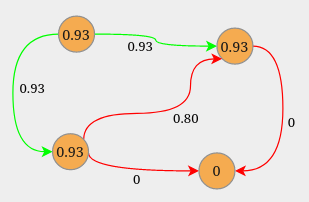
\includegraphics[width=\textwidth]{img/graph-example2-3.png}
				\caption{Relaxed solution}
				\label{fig:img/graph-example1-3.png}
			\end{subfigure}
		\end{center}
		\caption{Model solution for a graph with a single thread, for $\alpha =
				0.3$}
	\end{figure}

\end{frame}

\begin{frame}[c]
	\frametitle{The datasets - negative edge fractions for contents}
	\begin{figure}
		\begin{center}
			\begin{subfigure}[b]{0.4\textwidth}
				\centering
				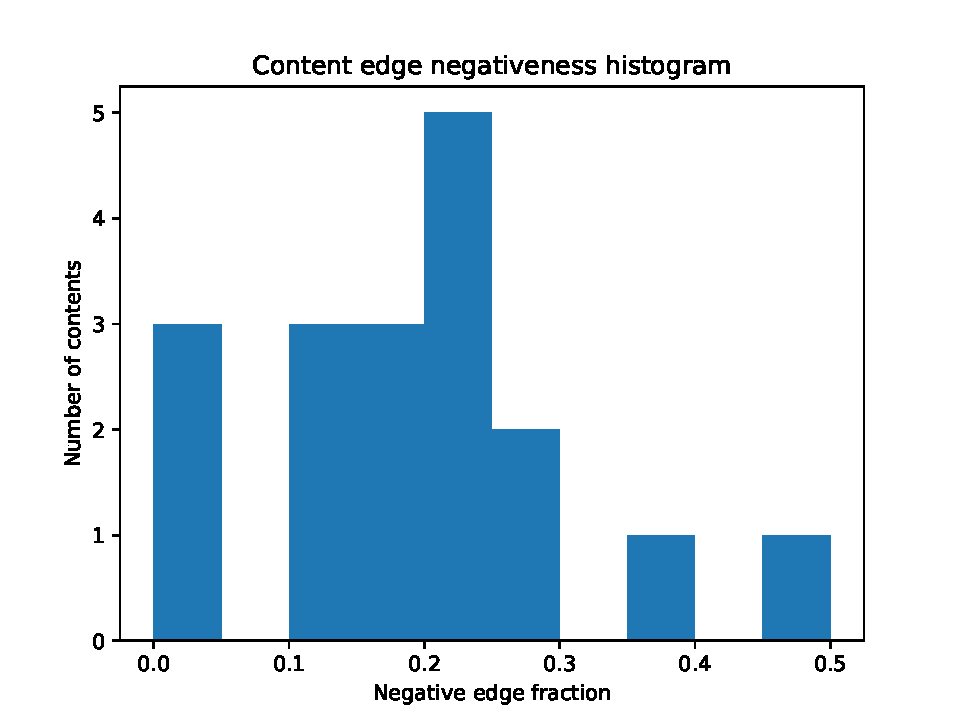
\includegraphics[width=\textwidth]{out/emanews200/neg-fraction-content-hist.pdf}
				\caption{@emanews}
				\label{fig:out/emanews200/neg-fraction-content-hist.pdf}
			\end{subfigure}
			\begin{subfigure}[b]{0.4\textwidth}
				\centering
				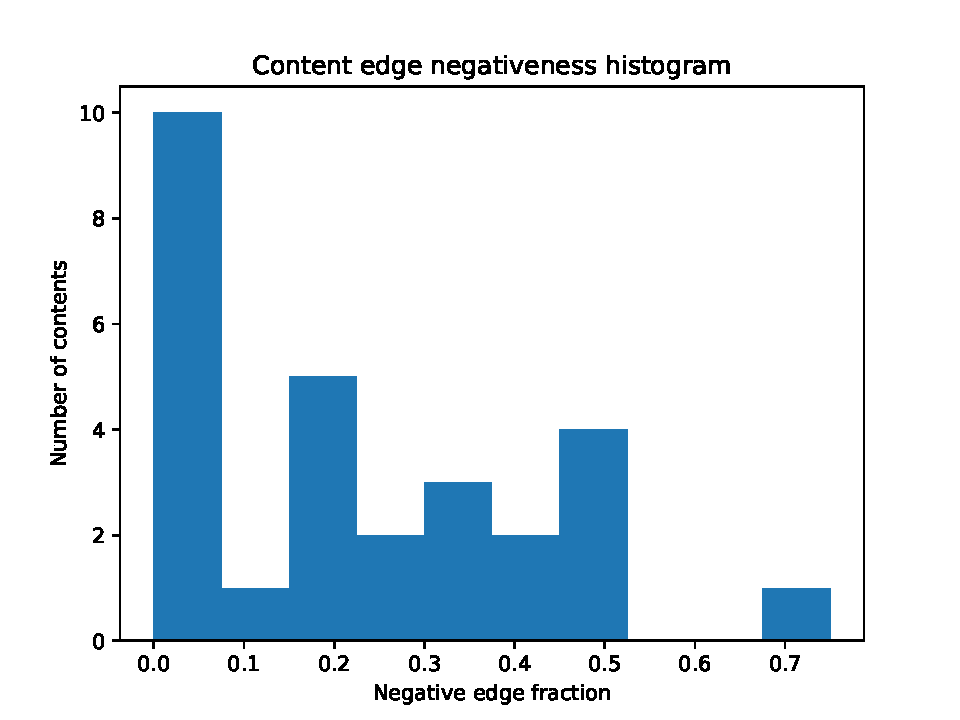
\includegraphics[width=\textwidth]{out/bbcscience200/neg-fraction-content-hist.pdf}
				\caption{@bbcscience}
				\label{fig:out/bbcscience200/neg-fraction-content-hist.pdf}
			\end{subfigure}
			\begin{subfigure}[b]{0.4\textwidth}
				\centering
				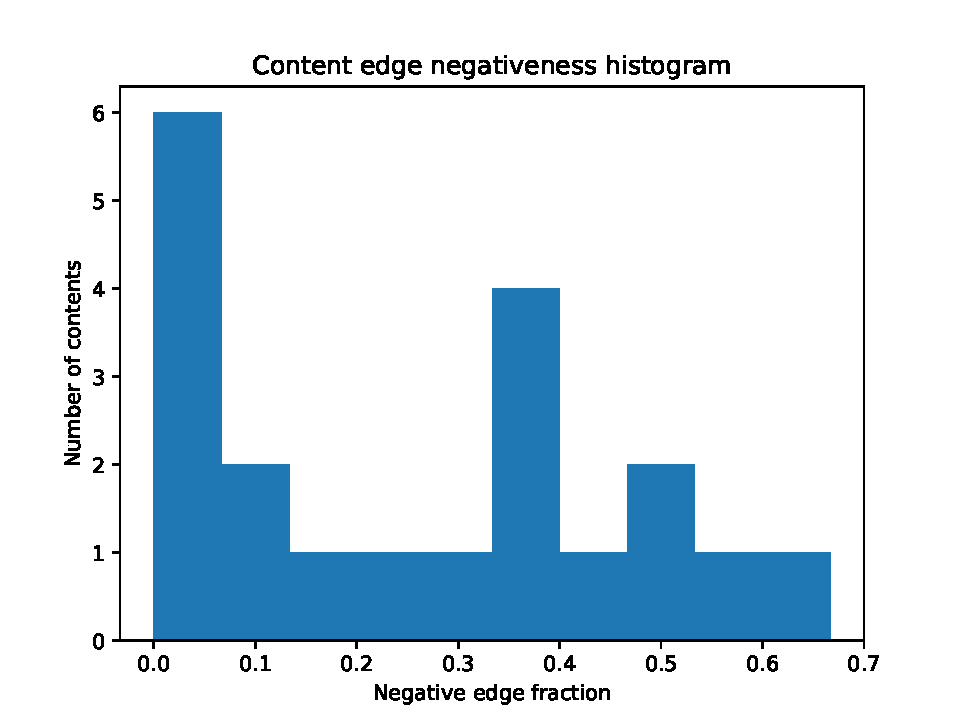
\includegraphics[width=\textwidth]{out/bbcentertainment200/neg-fraction-content-hist.pdf}
				\caption{@bbcentertainment}
				\label{fig:out/bbcscience200/neg-fraction-content-hist.pdf}
			\end{subfigure}
			\begin{subfigure}[b]{0.4\textwidth}
				\centering
				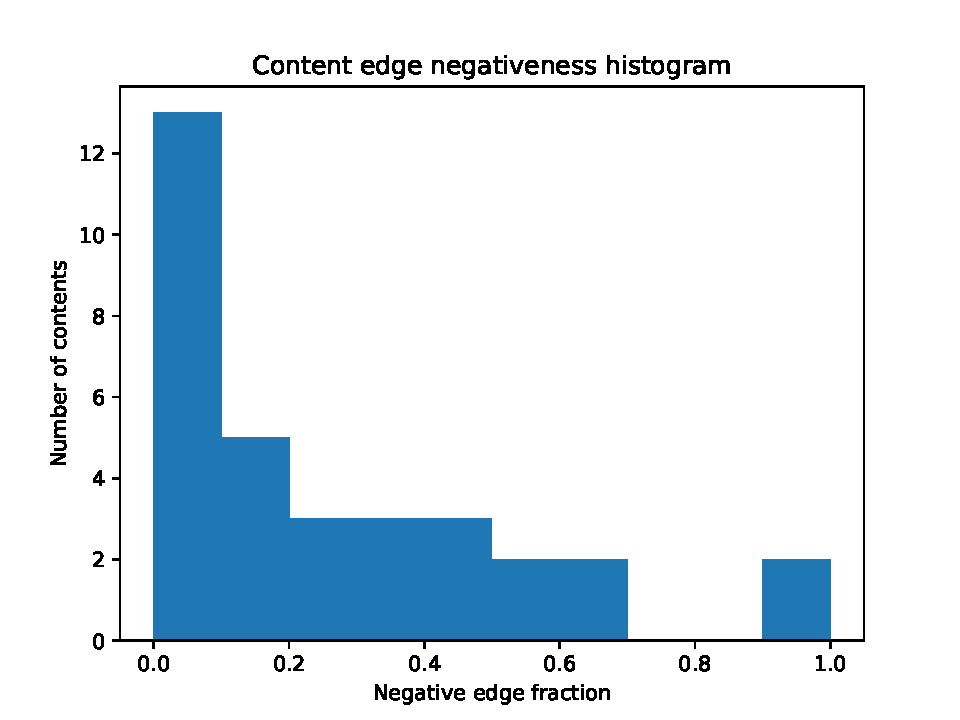
\includegraphics[width=\textwidth]{out/bbctech200/neg-fraction-content-hist.pdf}
				\caption{@bbctech}
				\label{fig:out/emanews200/neg-fraction-content-hist.pdf}
			\end{subfigure}
		\end{center}
	\end{figure}

\end{frame}


\begin{frame}[c]
	\frametitle{An initial implementation - results}
	\begin{itemize}
		\item Beta algorithm was repeated $ \sqrt{n}$ times for a graph with $n$ nodes
	\end{itemize}

	\begin{table}[htpb]
		\centering
		\caption{Echo chamber scores, greedy approach}
		\begin{tabular}{c|c|c|c|c}
			\textbf{Source}     & {|V|}                   & {|E|}
			                    & $(\xi_\beta(G), \beta)$ &
			$\xi_{peel} (G)$                                                       \\
			\hline
			{@emanews}          & {1226}                  & {1842} & (0, *)    & 0 \\
			{@bbcscience}       & {477}                   & {388}  & (3, 0.9)  & 7 \\
			{@bbcentertainment} & {220}                   & {183}  & (21, 1.0)
			                    & 16                                               \\
			{@bbctech}          & {793}                   & {719}  & (101, *)
			                    & 107                                              \\
		\end{tabular}
	\end{table}
	\begin{table}[htpb]
		\centering
		\caption{Echo chamber scores, MIP approaches}
		\begin{tabular}{c|c|c|c}
			\textbf{Source}     & $\xi_{MIP}(G) $ & $\xi_{MIPr}(G)$ &
			$\xi_{MIPr\_alg}(G)$                                          \\
			\hline
			{@emanews}          & 0               & 1.43            & 0   \\
			{@bbcscience}       & 7               & 10.76           & 7   \\
			{@bbcentertainment} & 34              & 41.69           & 34  \\
			{@bbctech}          & 309             & 326.63          & 309 \\
		\end{tabular}
	\end{table}
\end{frame}

\begin{frame}[c]
	\frametitle{Computing exactly the score - relaxation algorithm counterexample}
	\begin{figure}[htpb]
		\centering
		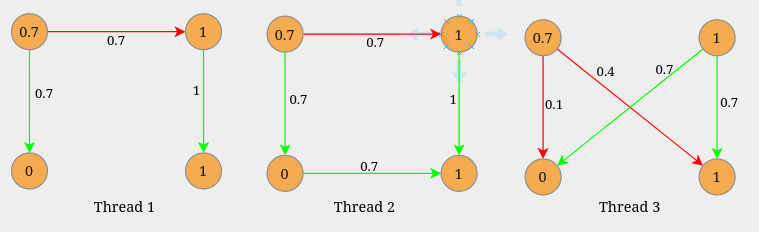
\includegraphics[width=0.8\linewidth]{img/counterexample.png}
		\caption{Small graph in which the algorithm may not find the
			optimum. The exact solution excludes the top-left vertex and scores
			5.}%
		\label{fig:img/counterexample}
	\end{figure}

\end{frame}

\begin{frame}[c]
	\frametitle{Echo Chamber Problem hardness}

	\begin{theorem}
		The Echo Chamber Problem is $\mathcal{NP}$-hard.
	\end{theorem}

\end{frame}

\end{document}
